% CHAPTER 4
\chapter {RESULTS}%and evaluation
\label {chp:results}
Contents here.

\section {Preliminary Analysis}
	\subsection {Manipulation Check}
Contents here.\\

\begin{table}[h]
\captionsetup{labelfont=bf, justification=justified,singlelinecheck=false}
\caption[CaptionforListofTables]{Caption}
\label {table:manipulationcheck}
\begin{tabularx}{1.0\textwidth}{lccl}
\hline
\multicolumn{1}{c}{} & \begin{tabular}[c]{@{}c@{}}Control Group \\ ($n$=50)\end{tabular} & \begin{tabular}[c]{@{}c@{}}Experimental Group\\ ($n$=51)\end{tabular} &  \\ \hline
\multicolumn{1}{c}{Scale Name} & \multicolumn{2}{c}{$M$ ($SD$)} & $t$(99) \\ \hline
IV & 2.64 (2.02) & 5.45 (1.72) & 7.53$^{\ast}$ \\
IV & 2.29 (1.62) & 4.39 (2.07) & 5.65$^{\ast\ast\ast}$ \\
IV & 2.30 (1.61) & 2.96 (1.95) & 1.86 \\ \hline
$^{\ast}p$ \textless .05, $^{\ast\ast\ast}p$ \textless .001 & \multicolumn{1}{l}{} & \multicolumn{1}{l}{} & \multicolumn{1}{l}{}
\end{tabularx}
\end{table}

\section {Primary Analysis}
Contents here. It was revealed that the players who were subjected to time pressure ($M = 5.38, SD = 1.02$) experienced more flow than the participants in the control group who were not ($M = 4.84, SD = 1.44$); $t(99) = 2.21, p = .030$ (See Table~\ref{table:primaryresults}). 

\begin{table}[h]
\captionsetup{labelfont=bf, justification=justified,singlelinecheck=false}
\caption[CaptionforListofTables]{Caption}
\label {table:primaryresults}
\begin{tabularx}{1.0\textwidth}{lccl}
\hline
\multicolumn{1}{c}{} & \begin{tabular}[c]{@{}c@{}}Control Group \\ ($n$=50)\end{tabular} & \begin{tabular}[c]{@{}c@{}}Experimental Group\\ ($n$=51)\end{tabular} &   \\ \hline
\multicolumn{1}{c}{Dependent variables} & \multicolumn{2}{c}{$M$ ($SD$)} & $t$ (99) \\ \hline
DV & 3.03 (1.31) & 3.37 (1.36) & 1.24 \\
DV & 4.83 (1.56) & 4.86 (1.40) & 0.11\\
DV & 3.82 (0.88) & 3.96 (0.90) & 0.76 \\
DV & 4.84 (1.44) & 5.38 (1.02) & 2.21$^{\ast}$ \\
DV & 3.52 (0.88) & 3.81 (0.95) & 1.62 \\
DV & 92.7 (17.4) & 94.5 (11.3) & 0.62 \\
DV & 4.83 (1.41) & 4.94 (1.01) & 0.46 \\
DV & 130.62 (39.4) & 110.49 (10.9) & 3.51$^{\ast\ast}$ \\ \hline
$^{\ast}p$ \textless .05, $^{\ast\ast}p$ \textless .01 & \multicolumn{1}{l}{} & \multicolumn{1}{l}{} & \multicolumn{1}{l}{}
\end{tabularx}
\end{table} 

Contents here. (See Table~\ref{table:gameendconditions}).

\begin{table}[H]
\captionsetup{labelfont=bf, justification=justified,singlelinecheck=false}
\caption[CaptionforListofTables]{Caption}
\label {table:gameendconditions}
\begin{tabular}{lcc}
\hline
\multicolumn{1}{c}{} & \begin{tabular}[c]{@{}c@{}}Control Group \\ ($n$=53)\end{tabular} & \begin{tabular}[c]{@{}c@{}}Experimental Group \\ ($n$=53)\end{tabular} \\ \hline
\multicolumn{1}{c}{Subgroups} & \multicolumn{2}{c}{$n$} \\ \hline
Subgroup & 50 & 29 \\
Subgroup  & 3 & 2 \\
Subgroup & - & 22 \\ \hline
\end{tabular}
\end{table}


One-Way between subjects ANOVA. However, there was a significant difference in perceived time pressure, flow and engagement at the $p<.05$ level for three conditions [$F(2,98) = 21.4, p < .001$ and $F(2,98) = 3.70, p = .028$ and $F(2,98) = 3.24, p = .043$ respectively] (See Table~\ref{table:anovaresults}).

\begin{table}[h]
\captionsetup{labelfont=bf, justification=justified,singlelinecheck=false}
\caption[CaptionforListofTables]{Caption}
\label {table:anovaresults}
\resizebox{\columnwidth}{!}{
\begin{tabular}{lcccccl}
\hline
 & \begin{tabular}[c]{@{}c@{}}Control Group \\ ($n$ = 53)\end{tabular} &  & \multicolumn{2}{c}{\begin{tabular}[c]{@{}c@{}}Experimental Group \\ ($n$ = 53)\end{tabular}} & \multicolumn{1}{l}{} & \multicolumn{1}{l}{} \\ \cline{2-2} \cline{4-5}
 & \begin{tabular}[c]{@{}c@{}}Successful \\ ($n$ = 50)\end{tabular} &  & \begin{tabular}[c]{@{}c@{}}Successful \\ ($n$ = 29)\end{tabular} & \begin{tabular}[c]{@{}c@{}}No Time \\ ($n$ = 22)\end{tabular} & \multicolumn{1}{l}{} & \multicolumn{1}{l}{} \\ \cline{2-5}
\multicolumn{1}{c}{} & \multicolumn{4}{c}{$M$} & $F$ (2,98) & Sig. \\ \hline
IV & 2.29 &  & 3.76 & 5.23 & 21.4 & .000$^{\ast\ast\ast}$ \\
DV & 3.03 &  & 3.20 & 3.56 & 1.23 & .30 \\
DV & 4.83 &  & 5.23 & 4.38 & 2.16 & .12 \\
DV & 3.82 &  & 3.83 & 4.12 & 0.96 & .39 \\
DV & 4.84 &  & 5.14 & 5.69 & 3.70 & .028$^{\ast}$ \\
DV & 3.52 &  & 3.60 & 4.10 & 3.24 & .043$^{\ast}$ \\
DV & 92.7 &  & 98.1 & 89.8 & 2.31 & .11 \\ 
DV & 4.83 &  & 4.93 & 4.97 & .11 & .89 \\ \hline
$^{\ast}p$ \textless .05, $^{\ast\ast\ast}p$\textless .001 & \multicolumn{1}{l}{} & \multicolumn{1}{l}{} & \multicolumn{1}{l}{} & \multicolumn{1}{l}{} & \multicolumn{1}{l}{} & \multicolumn{1}{l}{}
\end{tabular}}
\end{table}

Post Hoc comparisons using the Tukey HSD test indicated that the mean scores of perceived time pressure for successful subgroup of control group ($M = 2.29, SD = 1.62$) were significantly lower from successful ($M = 3,76, SD = 2.08$) and no time subgroups of experimental group ($M = 5.23, SD = 1.77$). (See Figure~\ref{fig:means}).

\begin{figure}[h]
\centering
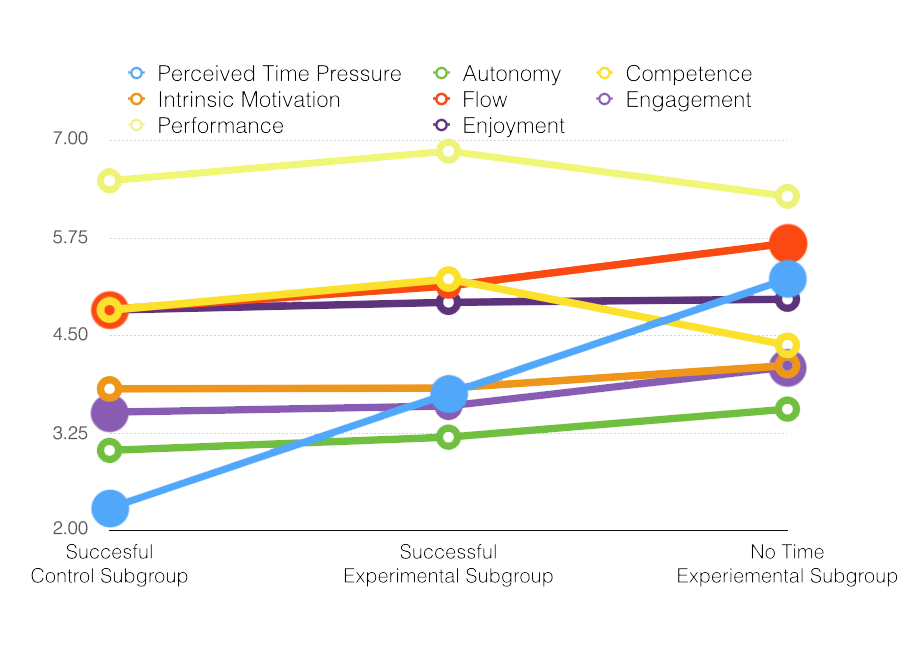
\includegraphics [width=.9\textwidth,clip]{images/Figure_6_Results}
\caption[CaptionforListofFigures]{Caption. \it {Note: Some note.}}
\label {fig:means}
\end{figure}

Although there was no significant difference in competence between both two main groups (control and experimental) and three subgroups, it approached significance between successful and no time subgroups of experimental group ($M = 5.23, SD = 1.22$ and $M = 4.38, SD = 1.48$ with $p = .10$, respectively). Furthermore, positive correlation between competence and performance [$r$ = .43, $n$ = 53, $p$ = .001] was revealed in the results of experimental group (See Table~\ref{table:correlationBygroup}).  

\begin{figure}[h]
\centering
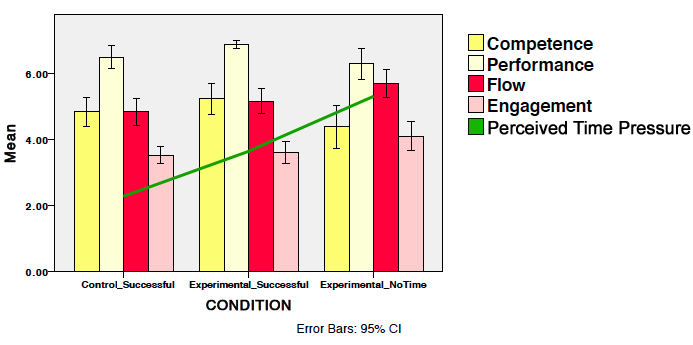
\includegraphics [width=1\textwidth,clip]{images/Figure_7_Discussion}
\caption[CaptionforListofFigures]{Caption}
\label {fig:subgroups}
\end{figure}

\begin{table}[h]
\captionsetup{labelfont=bf, justification=justified,singlelinecheck=false}
\caption[CaptionforListofTables]{Caption}
\label {table:correlationBygroup}
\resizebox{\columnwidth}{!}{
\begin{tabular}{llllllllll}
\hline
 &  & \multicolumn{8}{c}{Control Group} \\ \cline{3-10} 
 &  & IV & DV & DV & \begin{tabular}[c]{@{}l@{}}Long \\ DV\end{tabular} & DV & DV & DV & DV \\ \cline{2-10} 
\multicolumn{1}{l|}{\multirow{8}{*}{\begin{sideways}Experimental Group\end{sideways}}} & IV & - & .31$^{\ast}$ & -.16 & .48$^{\ast\ast}$ & .21 & .30$^{\ast}$ & -.04 & .06 \\
\multicolumn{1}{l|}{} & DV & .17 & - & .32$^{\ast}$ & .53$^{\ast\ast}$ & .05 & .25 & .01 & .46$^{\ast\ast}$ \\
\multicolumn{1}{l|}{} & DV & -.13 & .33$^{\ast}$ & - & .26 & .33$^{\ast}$ & .34$^{\ast}$ & .26 & .56$^{\ast\ast}$ \\
\multicolumn{1}{l|}{} & Long DV & .43$^{\ast\ast}$ & .41$^{\ast\ast}$ & .09 & - & .54$^{\ast\ast}$ & .61$^{\ast\ast}$ & -.10 & .77$^{\ast\ast}$ \\
\multicolumn{1}{l|}{} & DV & .12 & .44$^{\ast\ast}$ & .14 & .38$^{\ast\ast}$ & - & .65$^{\ast\ast}$ & .10 & .42$^{\ast\ast}$ \\
\multicolumn{1}{l|}{} & DV & .27 & .63$^{\ast\ast}$ & .15 & .61$^{\ast\ast}$ & .67$^{\ast\ast}$ & - & .06 & .46$^{\ast\ast}$ \\
\multicolumn{1}{l|}{} & DV & .08 & -.10 & .43$^{\ast\ast}$ & -.11 & -.30$^{\ast}$ & -.23 & - & -.07 \\
\multicolumn{1}{l|}{} & DV & .14 & .41$^{\ast\ast}$ & .35$^{\ast\ast}$ & .66$^{\ast\ast}$ & .31$^{\ast}$ & .38$^{\ast\ast}$ & -.04 & - \\ \cline{2-10} 
 & $^{\ast}p$ \textless .05, $^{\ast\ast}p$\textless .01 &  &  &  &  &  &  &  & \\ 
 & \multicolumn{9}{l}{\textit{Note.} $n$ = 53 \textit{for both groups. Correlations for Experimental Group lies on the lower part of the diagonal, correlations for Control}} \\ 
 & \multicolumn{9}{l}{\textit{Group lies on the upper part of the diagonal.}}
\end{tabular}}
\end{table}


\begin{table}[H]
\captionsetup{labelfont=bf, justification=justified,singlelinecheck=false}
\caption[CaptionforListofTables]{Caption}
\label {table:correlation}
\resizebox{\columnwidth}{!}{
\begin{tabular}{lllllllll}
\hline
 & \begin{tabular}[c]{@{}l@{}}Long \\ IV\end{tabular} & DV & DV & \begin{tabular}[c]{@{}l@{}}Long \\ DV\end{tabular} & DV & DV & DV & DV \\ \hline
Long IV & - &  &  &  &  &  &  &  \\
DV & .27$^{\ast\ast}$ & - &  &  &  &  &  &  \\
DV & -.13 & .32$^{\ast\ast}$ & - &  &  &  &  &  \\
Long DV & .44$^{\ast\ast}$ & .48$^{\ast\ast}$ & .18 & - &  &  &  &  \\
DV & .25$^{\ast}$ & .24$^{\ast}$ & .26$^{\ast\ast}$ & .48$^{\ast\ast}$ & - &  &  &  \\
DV & .33$^{\ast\ast}$ & .46$^{\ast\ast}$ & .24$^{\ast}$ & .62$^{\ast\ast}$ & .65$^{\ast\ast}$ & - &  &  \\
DV & .05 & -.03 & .33$^{\ast\ast}$ & -.09 & -.02 & -.06 & - &  \\
DV & .11 & .43$^{\ast\ast}$ & .48$^{\ast\ast}$ & .72$^{\ast\ast}$ & .39$^{\ast\ast}$ & .42$^{\ast\ast}$ & -.06 & - \\ \hline
\textit{Note.} $n$ = 106. &  &  &  &  &  &  &  & \\
 \multicolumn{9}{l}{$^{\ast}p$ \textless .05, $^{\ast\ast}p$\textless .01}
\end{tabular}}
\end{table}

\section {Discussion}
Contents here. (See Table~\ref{table:anovaresults}).  (See Figure~\ref{fig:means}).

